\documentclass[tikz,border=10pt]{standalone}

\usepackage{tikz}
\usepackage{tikz-cd}
\usetikzlibrary{arrows,automata,shapes,positioning,decorations.pathmorphing}
% \tikzset{->,>=stealth',auto}
\tikzset{->,auto}
\tikzset{>={Latex[width=2mm,length=2mm]}}
\tikzset{state/.style={shape=circle, draw, fill=white, initial text=,
    inner sep=.5mm, minimum size=2mm}}
\tikzset{state with output/.style={shape=rectangle split, rectangle
    split parts=2, draw, fill=white,
    initial text=, inner sep=1mm}}
\tikzset{every node={font=\footnotesize}}

\begin{document}
  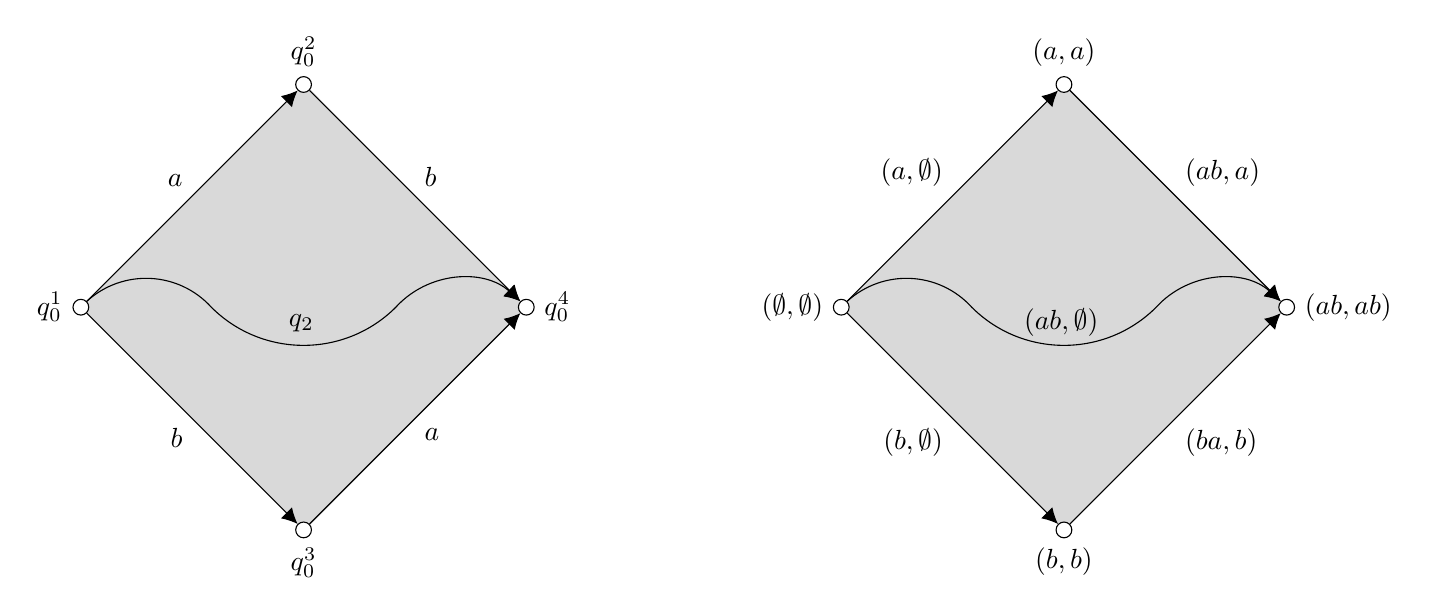
\begin{tikzpicture}[node distance=4cm, align=center]
    \title{ST-structure}
    \path[fill=black!15] (0,0) to (2.84,-2.84) to (5.65,0) to (2.84,2.84) to (0,0);
    \path[fill=black!15] (9.65,0) to (12.49,-2.84) to (15.3,0) to (12.49,2.84) to (9.65,0);

    \node(q1)[state] [label=left:{$q^1_0$}]                        {};
    \node(q2)[state] [above right of=q1, label=above:{$q^2_0$}]    {};
    \node(q3)[state] [below right of=q1, label=below:{$q^3_0$}]    {};
    \node(q4)[state] [below right of=q2, label=right:{$q^4_0$}]    {};
    
    \node(q11)[state] [right of=q4, label=left:{($\emptyset, \emptyset$)}]                        {};
    \node(q22)[state] [above right of=q11, label=above:{($a,a$)}]    {};
    \node(q33)[state] [below right of=q11, label=below:{($b,b$)}]    {};
    \node(q44)[state] [below right of=q22, label=right:{($ab,ab$)}]    {};
    
    \node(q13) [left of=q4] {};
    \node(q12)[right of=q1] {};
    
    \node(q113) [left of=q44] {};
    \node(q112)[right of=q11] {};
    
    \node(text) at (2.8,-0.2) {$q_2$};
    \node(text2) at (12.45,-0.2) {($ab,\emptyset$)};
    
    %\draw [->][draw=black] (q1) to [out =40,in =110] node {} (q13) to [out=-70,in=-150] (q4);
    \draw [->][draw=black] (q1) to [bend left=45] (q13.center) to [bend right=45] (q12.center) to [bend left=45] (q4);
    \draw [->][draw=black] (q11) to [bend left=45] (q113.center) to [bend right=45] (q112.center) to [bend left=45] (q44);
%    \draw [->][draw=black] (q1) to [out=70,in=110] node {} (q13) to [out=-70, in=-150] (q4);
    
    \draw [->][draw=black] (q1) to node [above left] {$a$} (q2);
    \draw [->][draw=black] (q1) to node [below left] {$b$} (q3);
    \draw [->][draw=black] (q2) to node [above right] {$b$} (q4);
    \draw [->][draw=black] (q3) to node [below right] {$a$} (q4);
    
    \draw [->][draw=black] (q11) to node [above left] {($a,\emptyset$)} (q22);
    \draw [->][draw=black] (q11) to node [below left] {($b, \emptyset$)} (q33);
    \draw [->][draw=black] (q22) to node [above right] {($ab, a$)} (q44);
    \draw [->][draw=black] (q33) to node [below right] {($ba, b$)} (q44);


  \end{tikzpicture}
\end{document}